\documentclass[10pt,a4paper]{article}
\usepackage{arabtex}
\usepackage[OT1,T1,LFE,LAE]{fontenc}
\usepackage[utf8]{inputenc}
\usepackage[arabic,english,farsi]{babel}
\usepackage{amsmath,amsfonts} % Math packages
\usepackage{amssymb}

\usepackage{multicol}

\usepackage{graphicx}
\usepackage{color}
\usepackage{float}
\usepackage{sidecap}
\usepackage{anysize}
\marginsize{2cm}{2cm}{2cm}{2cm}

\usepackage{listings}

\usepackage{appendix}

\usepackage[colorlinks=true,plainpages=true,citecolor=blue,linkcolor=blue,urlcolor=cyan]{hyperref}

%%% Equation and float numbering
\numberwithin{equation}{section}
\numberwithin{figure}{section}
\numberwithin{table}{section}


\newcommand{\horrule}[1]{\rule{\linewidth}{#1}} 	% Horizontal rule

\newcommand{\titleText}{STP and Switch \\ Laboratory Manual}

\title{
\normalsize In the name of Allah\\
\vspace{10pt}
\LARGE\FR{بسم \allah الرحمن الرحیم}
\vspace{10pt}
\begin{center}
	%	\newcommand{\HRule}{\rule{\linewidth}{0.5mm}}
	\begin{minipage}{0.48\textwidth} \begin{flushleft}
			
\includegraphics[height=64pt,width=64pt]{../img/logo.png}
	\end{flushleft}\end{minipage}
	\begin{minipage}{0.48\textwidth} \begin{flushright}
			
\includegraphics[height=64pt]{../img/eng-logo.png}
	\end{flushright}\end{minipage}
\end{center}
\vspace*{-64pt}
%	\horrule{0.5pt} \\[0.4cm]
	\huge \titleText\\
\vspace{40pt}
%	\horrule{2pt} \\[0.5cm]
}
\author{
	\huge University of Tehran\\
	\LARGE \FR{دانشگاه تهران}\\
	\\
	\LARGE School of Electrical and Computer Engineering\\
	\FR{دانشکده مهندسی برق و کامپیوتر}\\
	\\
	\Large Computer Network Lab\\
	\FR{آزمایشگاه شبکه‌های کامپیوتری}\\
	\\
	\\
	\\
	\normalfont
	Dr. Ahmad Khonsari - \FR{احمد خونساری}\\
	\href{mailto:a_khonsari@ut.ac.ir}{a\_khonsari@ut.ac.ir}\\
	\\
	\normalsize
	Amir Haji Ali Khamseh'i - \FR{امیر حاجی علی خمسه‌ء}\\
	\href{mailto:khamse@ut.ac.ir}{khamse@ut.ac.ir}\\
	\\
	\normalsize
	Sina Kashi pazha - \FR{سینا کاشی پزها}\\
	\href{mailto:sina\_kashipazha@ut.ac.ir}{sina\_kashipazha@ut.ac.ir}\\
	\\
	\normalsize
	Amirahmad Khordadi - \FR{امیر احمد خردادی}\\
	\href{mailto:a.a.khordadi@ut.ac.ir}{a.a.khordadi@ut.ac.ir}
}

\date{\vspace{30pt}\today\\\vspace{10pt}{\selectlanguage{farsi}\today}}

\usepackage{fancyhdr} 
\pagestyle{fancy}
%\pagestyle{fancyplain}
\fancyhf{}
\fancyhead[L]{\footnotesize Computer Network Lab \\ \FR{آزمایشگاه شبکه‌های کامپیوتری}}
\fancyhead[R]{\footnotesize \titleText}
\fancyfoot[R]{\footnotesize School of Electrical and Computer Engineering\\\FR{دانشکده مهندسی برق و کامپیوتر}}
\fancyfoot[C]{\thepage}
\fancyfoot[L]{\footnotesize University of Tehran \\ \FR{دانشگاه تهران}}
\renewcommand{\footrulewidth}{0.8pt}
\renewcommand{\headrulewidth}{1pt}			% Remove header underlines
\renewcommand{\footrulewidth}{1pt}				% Remove footer underlines
\setlength{\headheight}{13.6pt}
 

\begin{document}
\selectlanguage{english}

%\vspace*{-1.5cm}
\maketitle


\pagebreak


\section{Introduction}
In this session, we try checking switch network loop in Mininet and after implement it on Cisco devices. At the end of this session you must able to config Cisco switch and router.

\subsection*{Requirement}
\begin{itemize}
    \item Mininet + bridge-utils
    \item Cisco Packet Tracer or physical switch \& router
\end{itemize}

\section{Topology Configuration}
    Create Mininet custom topology like Figure \ref{fig:topology} with link delay $ 1 ms $.\\
    \textit{run mininet with argument: }\textbf{-{}-switch lxbr,stp=1 -{}-link tc}

    \begin{itemize}
        \setlength{\itemindent}{30pt}
        \item [bash>] run \textbf{sudo mn $\cdots$ -{}-switch lxbr,stp=1 -{}-link tc}
        \item [bash>] run \textbf{wireshark \&} on host (mininet) immediately
        \item [mininet] \textbf{pingall}
    \end{itemize}
    
\begin{figure}[H]
    \centering
    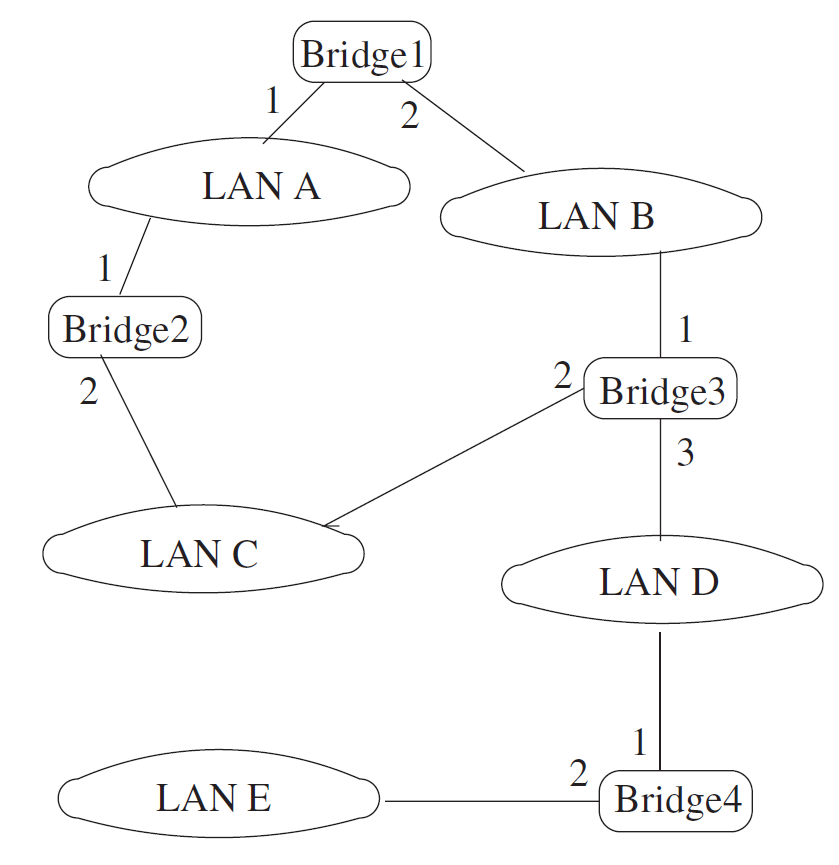
\includegraphics[height=192pt]{img/fig1.png}
    \caption{Topology}
    \label{fig:topology}
\end{figure}

    Whats happening?\\
    Wait for 30 sec. Now rerun \textbf{pingall} command.
    Whats happening? Explain?

    \subsection{Report}
    Submit the gratuitous ARP sent by the host and switch. What in \textbf{STP} frame?\\
    From the output of \textbf{show bridge}, identify which bridge ports are blocked, and which ports are in the forwarding state for each bridge.

\begin{figure}[H]
    \centering
    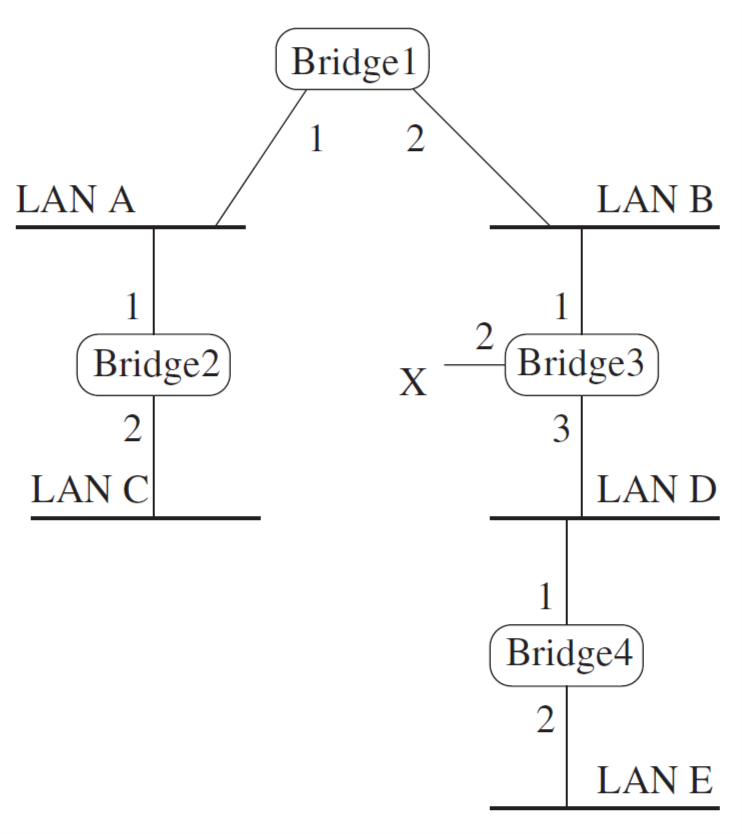
\includegraphics[height=160pt]{img/fig1-2.png}
    \caption{Corresponding tree for Figure \ref{fig:topology} with the loop removed}
    \label{fig:topology-simple}
\end{figure}

\section{Cisco}
    Create new project in Cisco Packet Tracer and configure topology in Figure \ref{fig:topology} by using 2960 switches and PC (Laptops) in toolbar.

(Use 2960 switch instead of bridge and set of two laptops and one switch instead of each LAN)\\
your configuration must be similar to the Figure \ref{fig:topology} in packet tracer.

\begin{figure}[H]
	\centering
    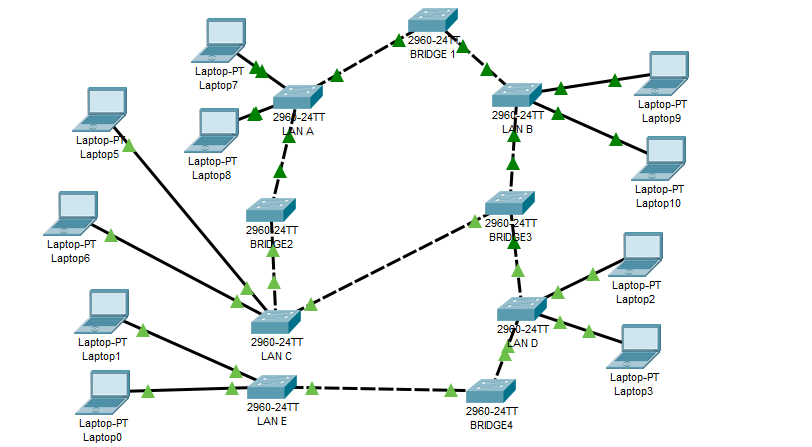
\includegraphics[height=100pt]{img/fig2.png}
    \caption{Implemented Topology in CPT}
\end{figure}

\subsection{Configuring IP address}
	Click  on each laptop and select Config tab then select the FastEthernet0 on the left vertical bar. set IP address for each laptop in 192.168.56.101 to 192.168.56.110 range. \\

	\begin{center}
        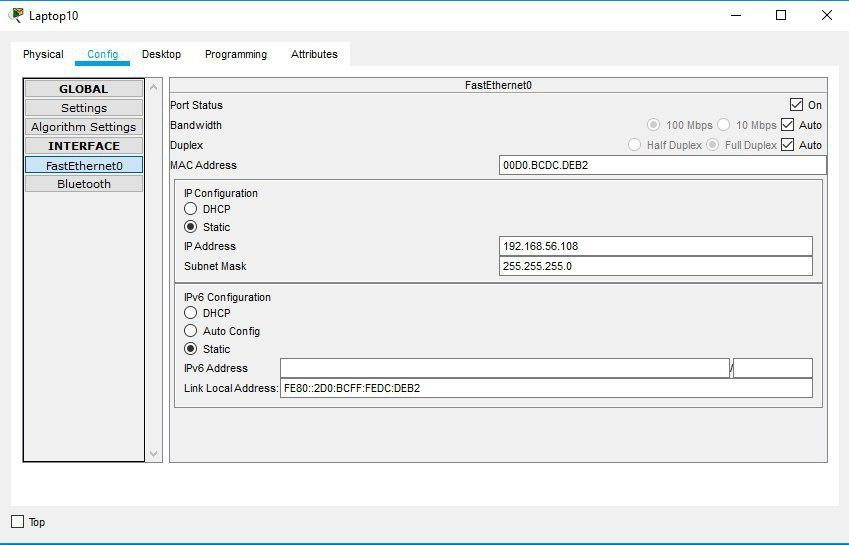
\includegraphics[height=200pt]{img/fig3.png}
    \end{center}
    
    \textbf{Ping} a laptop in LAN D by a laptop in LAN A.

\subsection*{How to Ping}

click on source laptop and select Desktop tab then select command prompt. You can ping destination laptop by its ip. 
\subsection*{Report}
	\begin{enumerate}
		\item show the ping result in your report.
		\item all Cisco command (not required to save graphical image. only report switch or router command)
	\end{enumerate}
    

    %\pagebreak
\subsection{Disabling Spanning-Tree Protocol}
	Click on each switch in your topology and select CLI(Command Line Interface) tab. Enter following commands for disabling STP.
    \begin{itemize}
        \setlength{\itemindent}{50pt}
		\item [Switch>] \textbf{enable}
		\item [Switch\#] \textbf{configure terminal \&}
		\item [Switch(config)\#] \textbf{no spanning-tree vlan 1-4096}
	\end{itemize}

    \subsection*{Report}
    \begin{enumerate}
        \item Repeat ping process from different source and show the ping result and explain the difference.

    \end{enumerate}
    
    %\pagebreak
\subsection{CLI help}
    Open a random router’s CLI and navigate through User EXEC, Privileged EXEC, Global Configuration and Interface Configuration Modes. In each mode, type ? to display a list of available commands and study these commands.

\subsubsection*{Report}
 Save the output of CLI when you type “?” in each mode and describe one command.
    

    %\pagebreak
\subsection{IP configuration}
    Configure the IP addresses of your workstation and the bridge interfaces as shown in Table 1 and Table 2.\\

    \begin{figure}[H]
        \centering
        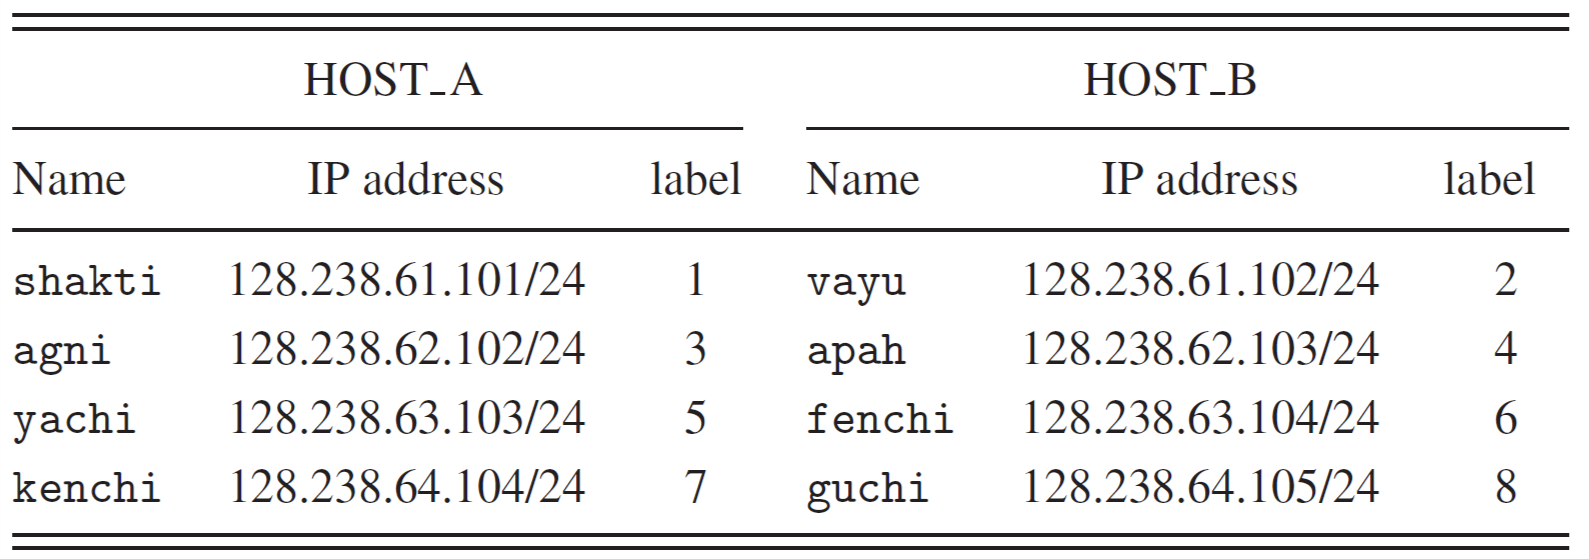
\includegraphics[width=0.6\textwidth]{img/table1.png}
        \caption{Table 1: Host IP addresses}
        \label{tbl:table1}
        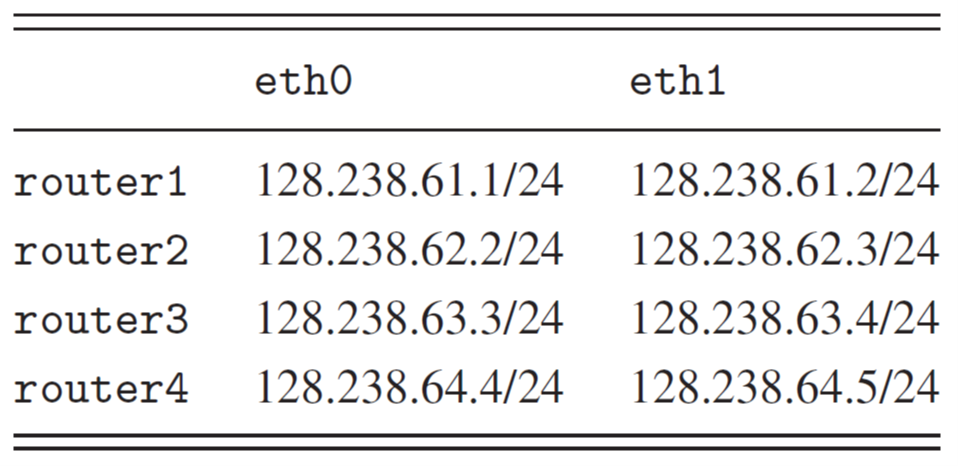
\includegraphics[width=0.4\textwidth]{img/table2.png}
        \caption{Table 2: Router IP addresses}
        \label{tbl:table2}
    \end{figure}

    ping two random hosts and capture ping packet.		

    \subsection*{Report}
    \begin{enumerate}
        \item What are the IP and MAC addresses of a packet that went from Host1 to the bridge? 
        \item What are the IP and MAC addresses of a packet that went from the router to Host2?
        \item Answer the same questions, but for the echo reply that was returned from Host2.
    \end{enumerate}

    %\pagebreak
\subsection{Bridge Protocol Data Unit}
   Capture 5 BPDU\footnote{see Appendix B} messages generated by bridges. Save the BPDUs for the lab report.
    \subsubsection*{Report}
    \begin{enumerate}
        \item How frequently (in seconds) does a bridge sends its BPDUs?
        \item Submit the five different BPDUs you saved. Identify the values of root ID, root path cost, bridge ID, and port ID for each BPDU.
    \end{enumerate}
    
\pagebreak
\subsection{Topology Configuration}
   In following Exercise we will use Figure \ref{fig:bridge-ex} as our network topology.You need to change the IP addresses of the bridge interfaces, as well as that of hosts.

\begin{figure}[H]
    \centering
    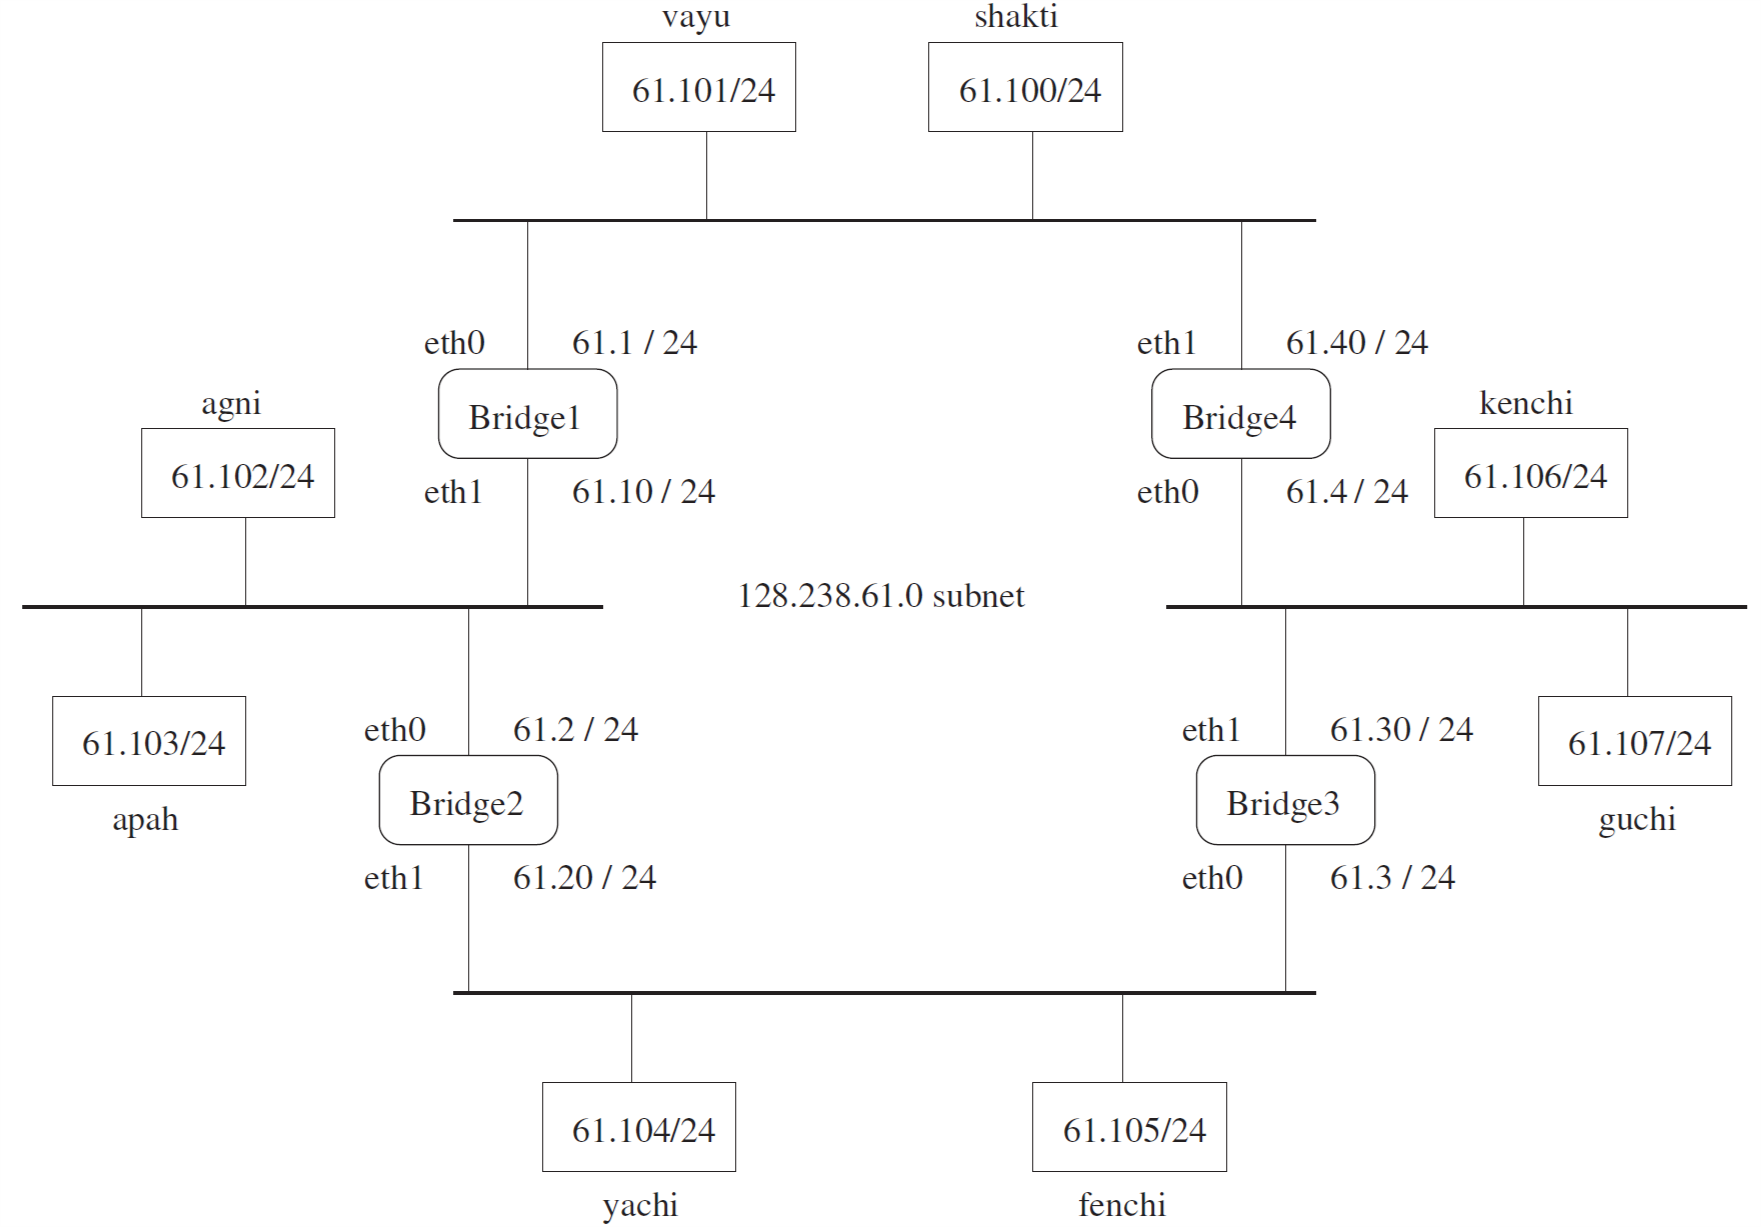
\includegraphics[width=0.8\textwidth]{img/fig4.png}
    \caption{Bridge experiment network}
    \label{fig:bridge-ex}
\end{figure}

% disable output
\iffalse
\section{Excercise 1}
   Get to the Privileged EXEC mode. Type show bridge to see the entries in the bridge forwarding database. \\ 
\\
Whenever you ping or telnet from your host to a host that is not in the table, observe how the filtering database in the bridge is expanded. \\
\\
You may use the clear bridge group command to remove any learned entries from the filtering database, if you see a full filtering database or if you want to repeat the above exercise. 

   \subsection*{Report}
    \begin{enumerate}
        \item From the output of show bridge, identify which bridge ports are blocked, and which ports are in the forwarding state for each bridge.
    \end{enumerate}

\section*{Excercise 2}
   Using tcpdump -ex ether multicast, capture the BPDU packet flowing on your network segment. \\
\\
Telnet to the hosts in the other three LAN segments and execute the above tcpdump command in the telnet window to collect BPDUs sent there. \\
\\
Login to each bridge to collect the show bridge outputs.

    \subsection*{Report}
    \begin{enumerate}
        \item Submit the four different BPDUs you saved. Identify the values of root ID, root path cost, bridge ID, and port ID for each BPDU. 
	    \item Based upon the initial BPDUs saved in Exercise 2, draw the spanning tree seen by the BPDUs. Identify the root ports and the root path cost (in hop counts) for each bridge. Identify the designated bridge and the designated port for each LAN segment. Identify the state of each bridge port (blocking or forwarding). 
        \item Don’t just assume that Bridge1 has the highest priority for the root bridge. Draw the spanning tree based upon your data (eight initial BPDUs). 
        \item Write the final BPDUs you collected using the three-tuple format: {root ID, root path cost, bridge ID}. 
        \item Once you have the spanning tree, justify it using the four final BPDUs collected in this exercise and/or the output of the show bridge command. 
    \end{enumerate}

\section*{Excercise 3}
  This exercise is performed by all the students together. First, send ping messages from apah to yachi, while tcpdump is running. Let the two programs run during this exercise. \\
Then, disconnect the cable from the ethernet0 port of Bridge2 from the hub, and type the time command on apah or yachi to get the current time. \\
Observe the ping and tcpdump windows. When the connection is reestablished, type the time command again. How long does it take the spanning tree algorithm to react to the change in the topology? \\
Once you can successfully reach other hosts, get to the bridges to run show bridge to collect the port states. Also collect BPDUs from all the LAN segments as you did in the previous exercise. \\
After every student has collected the required data, connect the cable to the original position. Again, measure the time it takes for the bridges to adapt to the new change. 


    \subsection*{Report}
    \begin{enumerate}
        \item Draw the new tree formed after the cable was disconnected, based on the BPDUs you collected in this exercise. Specify the state of each bridge port. 
    \end{enumerate}

\section*{Excercise 4}
 You can also configure a router using the web browser UI. To enable the web server, login to the router and execute ip http server in the Global Configuration mode. \\
Next, start a web browser (e.g., Mozilla in Linux, or Hotjava in Solaris) in your host, and enter the IP address of the router interface. When prompted, enter el537 for password, and leave the User Name field blank.Then you can browse the router configuration web pages and configure the router there. 
\fi

\appendix
\section*{Appendices}
\addcontentsline{toc}{section}{Appendices}
\renewcommand{\thesubsection}{\Alph{subsection}}

\subsection{Cisco IOS configuration modes}
\begin{figure}[H]
    \centering
    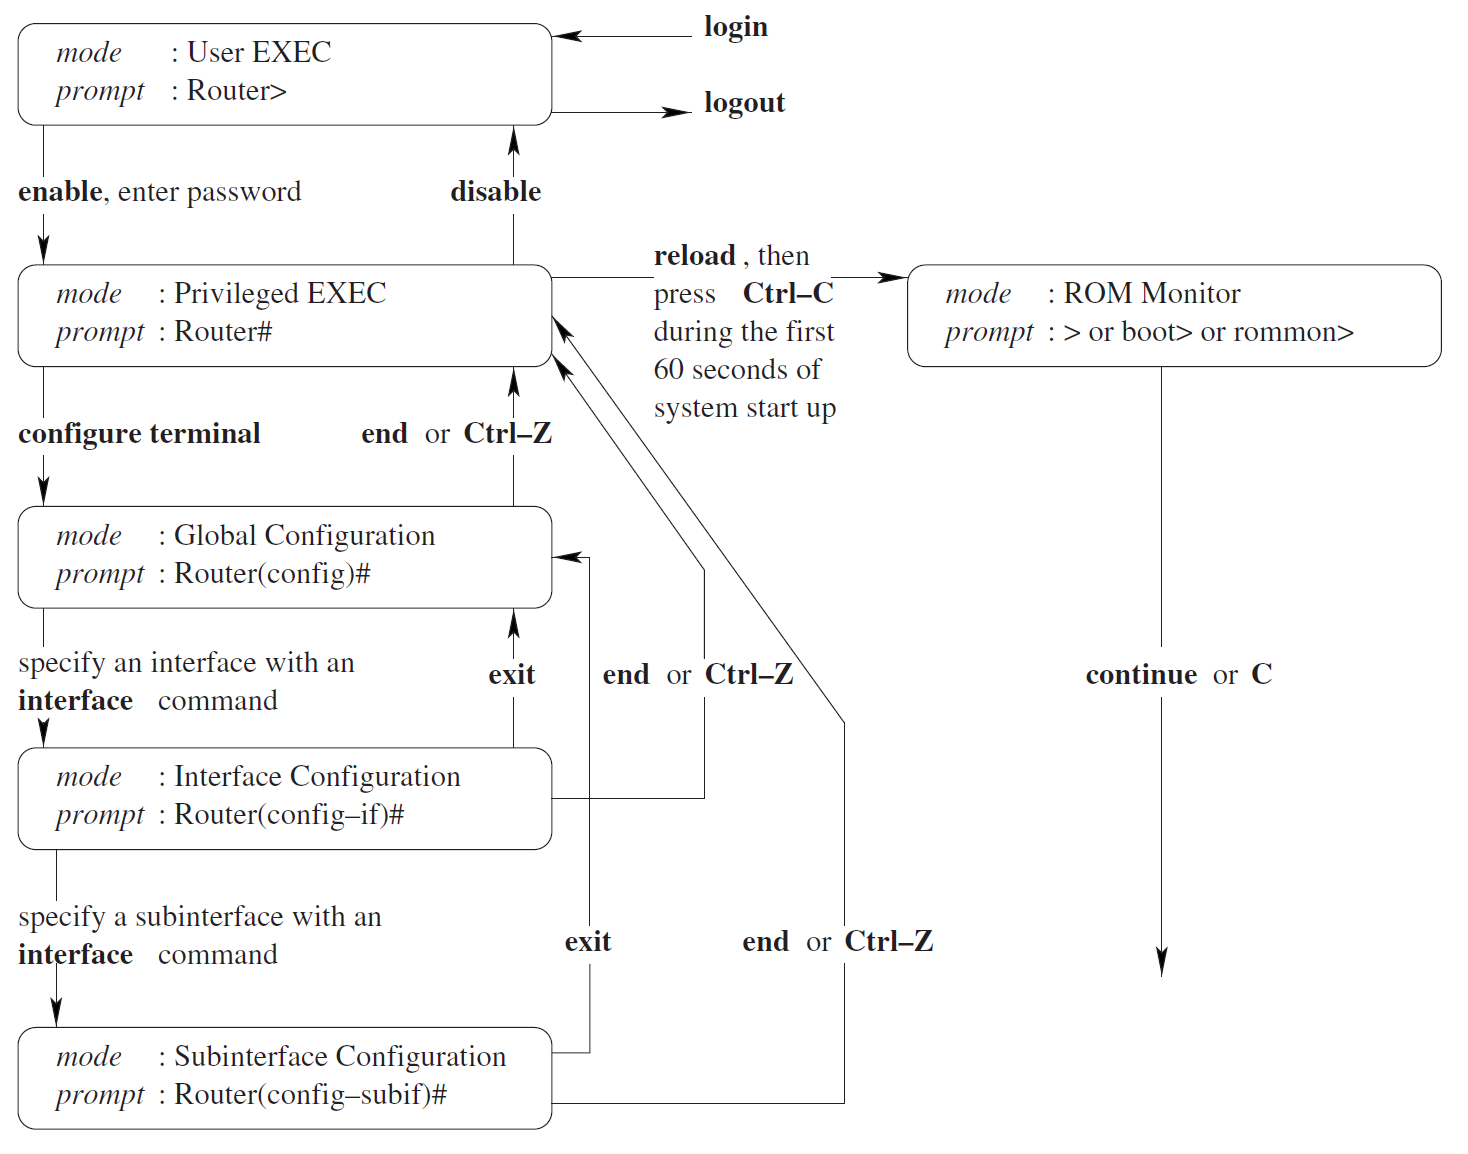
\includegraphics[width=\textwidth]{img/appendix-ios.png}
    \caption{Navigating through the Cisco IOS configuration modes}
\end{figure}
Reference: TCP/IP Essential
\subsection{BPDU}
\begin{figure}[H]
    \centering
    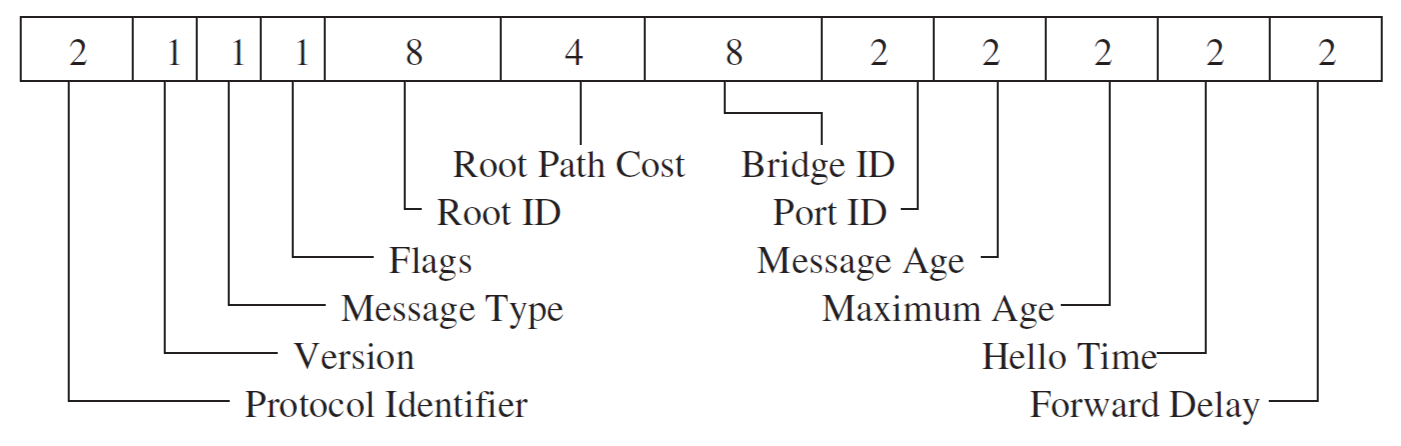
\includegraphics[width=\textwidth]{img/bpdu.png}
    \caption{BPDU message format. The numbers indicate the field length in byte.}
\end{figure}

\end{document}